\documentclass[]{standalone}
\usepackage[utf8]{inputenc}
\usepackage[american]{circuitikz}
\usetikzlibrary{arrows,shapes,calc,positioning}

\usepackage{graphicx}

\newcommand{\myscope}[2] % #1 = name , #2 = rotation angle
{\draw[thick,rotate=#2] (#1) circle (12pt)
 (#1) ++(-0.35,-0.1) -- ++(0.3,0.3) --++(0,-0.3)-- ++(0.3,0.3) --++(0,-0.3);
}

\begin{document}

\pgfmathsetmacro\circuitheight{5}
\pgfmathsetmacro\circuitwidth{5}

\begin{circuitikz}[scale=1]
  \node at (2.5,2.5) {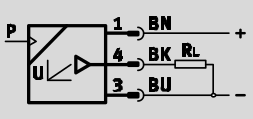
\includegraphics[width=3cm]{pressure-transmitter.png}};
  \draw (0,0) to[V, label=18V] (0, \circuitheight) to[short, -o] ++(\circuitwidth, 0); 
  \draw (3.6,5) to [short,-*] (3.6, 2.8);
  \draw (3.6,0) to [short,-*] (3.6, 2.07);
  \draw (0,0) to [short, -o] ++(\circuitwidth, 0); 

  \draw (3.6,2.46) to[short,*-] ++(1.3, 0) to[sV, color=white, name=S] (4.9, 0);
  \myscope{S}{0}
\end{circuitikz}
\end{document}
